% Diagnostic Assist: take-home submission.
% Build (XeLaTeX, for the system fonts and Unicode text):
%   xelatex submission.tex && xelatex submission.tex
\documentclass[11pt,a4paper]{article}

\usepackage[a4paper,margin=2.3cm,top=2.3cm,bottom=2.4cm,headsep=0.9cm]{geometry}
\usepackage{amsmath}
\usepackage{fontspec}
\usepackage{unicode-math}
\setmainfont{Charter}
\setsansfont{Helvetica Neue}
\setmonofont{Menlo}[Scale=0.82]
\setmathfont{latinmodern-math.otf}
\usepackage{microtype}
\usepackage[table]{xcolor}
\usepackage{booktabs,tabularx,array,longtable}
\usepackage{ragged2e}
\usepackage{enumitem}
\usepackage{titlesec}
\usepackage{fancyhdr}
\usepackage{fancyvrb}
\usepackage{tikz}
\usetikzlibrary{positioning,arrows.meta,calc,fit,backgrounds}
\usepackage{parskip}
\usepackage[hidelinks]{hyperref}
\usepackage{bookmark}

% ---------------------------------------------------------------- colours
\definecolor{accent}{HTML}{1F4E79}
\definecolor{muted}{HTML}{5B6573}
\definecolor{hair}{HTML}{C9CED6}
\definecolor{wash}{HTML}{F2F5F9}
\definecolor{todo}{HTML}{B3261E}

% ---------------------------------------------------------------- layout
\setlength{\parskip}{0.55em}
\setlist{nosep,leftmargin=1.4em,topsep=0.2em,itemsep=0.2em}
\setlist[enumerate]{leftmargin=1.6em}
\renewcommand{\arraystretch}{1.25}
\setlength{\tabcolsep}{5pt}
\setlength{\emergencystretch}{2.5em}
\setlength{\LTpre}{0.4em}
\setlength{\LTpost}{0.2em}
\setlength{\LTleft}{0pt}
\setlength{\LTright}{0pt}

\titleformat{\section}{\sffamily\Large\bfseries\color{accent}}{\thesection}{0.6em}{}
\titleformat{\subsection}{\sffamily\large\bfseries}{\thesubsection}{0.6em}{}
\titlespacing*{\section}{0pt}{1.5em}{0.45em}
\titlespacing*{\subsection}{0pt}{1.1em}{0.3em}

\pagestyle{fancy}
\fancyhf{}
\fancyhead[L]{\sffamily\footnotesize\color{muted}Diagnostic Assist\enspace·\enspace take-home submission}
\fancyhead[R]{\sffamily\footnotesize\color{muted}\thepage}
\renewcommand{\headrulewidth}{0.4pt}
\renewcommand{\headrule}{{\color{hair}\hrule width\headwidth height\headrulewidth}}

% ---------------------------------------------------------------- helpers
\newcommand{\code}[1]{\nolinkurl{#1}}
\newcommand{\ra}{\ensuremath{\rightarrow}}
\newcommand{\about}{\ensuremath{\sim}}
\newcolumntype{P}[1]{>{\RaggedRight\arraybackslash}p{#1}}
\newcolumntype{R}[2]{>{\RaggedRight\arraybackslash}p{\dimexpr(\linewidth-#1-2\tabcolsep*#2)/#2\relax}}

% Start a new page unless #1 lines still fit (keeps a heading with what follows).
\makeatletter
\newcommand{\needlines}[1]{\par\begingroup\dimen@=#1\baselineskip\dimen@ii=\pagegoal\advance\dimen@ii by -\pagetotal
  \ifdim\dimen@>\dimen@ii\ifdim\dimen@ii>\z@\vfil\fi\break\fi\endgroup}
\makeatother

\newsavebox{\calloutbox}
\newenvironment{callout}[1][accent]
  {\def\calloutcolor{#1}\par\smallskip\noindent
   \begin{lrbox}{\calloutbox}\begin{minipage}{\dimexpr\linewidth-2\fboxsep-11pt\relax}}
  {\end{minipage}\end{lrbox}%
   \colorbox{\calloutcolor!6}{\textcolor{\calloutcolor}{\vrule width 2.5pt}\hspace{8.5pt}\usebox{\calloutbox}}%
   \par\smallskip}

\fvset{fontsize=\small,frame=single,rulecolor=\color{hair},framesep=2.5mm,xleftmargin=0pt}

\hypersetup{pdftitle={Diagnostic Assist: take-home submission},pdfsubject={Diagnostic Assist take-home}}

% ================================================================ document
\begin{document}

\thispagestyle{empty}
\begin{center}
  {\sffamily\bfseries\fontsize{24}{28}\selectfont\color{accent}Diagnostic Assist}\\[0.5em]
  {\sffamily\large Take-home submission}\\[0.3em]
  {\sffamily\small\color{muted}October 2026}
\end{center}
\vspace{0.2em}

\begin{callout}
{\sffamily\bfseries In short}\par\smallskip
\begin{itemize}[leftmargin=1.1em]
  \item \textbf{The product.} A panel in the dispatcher's case screen. It shows the likely root causes with a probability for each, asks one useful question at a time, and suggests which parts to put on the van. The technician continues the same session on site.
  \item \textbf{The main decision.} \emph{The LLM reads, statistics decide.} An LLM turns old closed cases into structured records. The probabilities are then counted from similar past cases. No model makes up a percentage.
  \item \textbf{The hard part.} The data has no root-cause labels. Everything depends on a cause list that does not exist yet, and mistakes in it are silent.
  \item \textbf{What I built.} The “label factory”: the Python pipeline that turns closed cases into that cause list. It has 63 tests and runs on the sample and on new cases (see \code{README.md}). I ran its extraction prompt through Claude Opus 5.5 on all 22 sample cases: the real output groups exactly like my hand labels, and it found one ambiguity in my prompt.
  \item \textbf{When I would stop.} If the counted probabilities do not clearly beat “load what usually breaks on this model” in a backtest (section~\ref{sec:works}).
\end{itemize}
\end{callout}

% ================================================================ 1
\section{The product}\label{sec:product}

\subsection{Who uses it}

The main user is the \textbf{dispatcher during the intake call}. This is where the parts for the van are chosen, so this is where a first-time fix is won or lost. The dispatcher can ask the customer questions, but only about things the customer can see, like a code on the display.

The second user is the \textbf{technician on site}. They open the same session on their phone. They can measure and open panels, and their results update the same list. When they finish, they tap the cause they actually found. That tap gives us the label the old data never had.

It is \textbf{not a chatbot}. Nobody on a phone call or in front of a broken machine has time to chat. The system suggests; the user taps.

\subsection{What the dispatcher sees}

\newcommand{\causerow}[5]{% y, pct, name, parts, colour
  \fill[#5, rounded corners=1pt] (0.45,#1-0.14) rectangle ++({#2*0.105},0.28);
  \node[anchor=east] at (5.55,#1) {#2\%};
  \node[anchor=west] at (5.75,#1) {#3};
  \node[anchor=west, font=\ttfamily\footnotesize] at (11.6,#1) {#4};}
\newcommand{\chip}[2]{\node[draw=accent!60, fill=accent!6, rounded corners=6pt, inner xsep=7pt, inner ysep=3.5pt, anchor=west] (#1) {#2};}

\begin{center}
\begin{tikzpicture}[font=\sffamily\small]
  \draw[draw=hair, fill=white, rounded corners=5pt] (0,0) rectangle (15.9,-7.15);
  \begin{scope}
    \clip[rounded corners=5pt] (0,0) rectangle (15.9,-7.15);
    \fill[wash] (0,0) rectangle (15.9,-0.7);
  \end{scope}
  \draw[hair] (0,-0.7) -- (15.9,-0.7);
  \node[anchor=west, font=\sffamily\bfseries] at (0.35,-0.35) {Case C-48590\enspace·\enspace CX-450\enspace·\enspace “no crank, dead panel”};

  \node[anchor=west, font=\sffamily\footnotesize\bfseries, text=muted] at (0.35,-1.1) {LIKELY CAUSES (61 similar CX-450 cases)};
  \node[anchor=west, font=\sffamily\footnotesize\bfseries, text=muted] at (11.6,-1.1) {PARTS USUALLY NEEDED};
  \causerow{-1.58}{38}{Main contactor failed}{CONTACTOR-M1}{accent!75}
  \causerow{-2.03}{24}{Battery flat / failed}{BATT-95AH}{accent!75}
  \causerow{-2.48}{15}{Frame ground strap loose}{— (no part)}{accent!75}
  \causerow{-2.93}{9}{Alternator not charging}{ALT-450}{accent!75}
  \causerow{-3.38}{6}{No fault found (intermittent)}{—}{accent!75}
  \causerow{-3.83}{8}{Other}{}{black!25}

  \draw[hair] (0.35,-4.22) -- (15.55,-4.22);
  \node[anchor=west] at (0.35,-4.62) {\textbf{Ask the customer:}\enspace Has the battery gone flat before, recently?};
  \begin{scope}[shift={(0.35,-5.2)}]
    \chip{a}{Yes, repeatedly}
    \begin{scope}[shift={($(a.east)+(0.25,0)$)}]\chip{b}{No, first time}\end{scope}
    \begin{scope}[shift={($(b.east)+(0.25,0)$)}]\chip{c}{Don't know}\end{scope}
  \end{scope}
  \node[anchor=east, text=muted] at (15.55,-5.2) {skip};

  \draw[hair] (0.35,-5.7) -- (15.55,-5.7);
  \node[anchor=west] at (0.35,-6.1) {\textbf{Van loadout:}\enspace {\ttfamily\footnotesize CONTACTOR-M1 + BATT-95AH} covers \textbf{83\%} of likely causes};
  \node[anchor=east, text=accent] at (15.55,-6.1) {edit};
  \node[anchor=west, text=muted] at (0.35,-6.65) {Why?\enspace C-48211 “Unit won't start at all. No lights on the control panel.”\enspace$\blacktriangleright$};
\end{tikzpicture}
\end{center}

\subsection{How it works, step by step}

\begin{enumerate}
  \item The case opens with the machine type. The dispatcher types what the customer says, in any language.
  \item In about a second, the panel shows the top five causes plus “Other”. Each has a probability, the parts it usually needs, and how many similar cases it is based on. If the machine type has few cases, a badge says the numbers come from the wider equipment family.
  \item Below the list there is one question, with tap answers including “Don't know”. Each answer re-ranks the list straight away. A few seconds later, an LLM pass fills in answers the customer already gave (for example “E207 on the display”), so the dispatcher never asks twice.
  \item \textbf{It stops} when no answer to any remaining question could change the parts on the van, or after three questions. The goal is the right parts on the van, not a confident guess.
  \item The panel suggests the smallest set of parts that covers at least 80\% of the probability. 80\% is a business setting: van stock against the cost of a second visit. The dispatcher edits and confirms.
  \item On site, the technician sees the same causes as a list of checks, ordered by probability divided by minutes to check. Quick checks come first.
\end{enumerate}

\subsection{Walkthrough: C-48590, “no crank, dead panel” (CX-450)}

The numbers are illustrative; the steps are real.

\begin{itemize}
  \item The dispatcher types “no crank, dead panel”. The panel above appears: contactor 38\%, battery 24\%, ground strap 15\%, alternator 9\%, no fault found 6\%. It is based on similar CX-450 cases such as C-48211 and C-48377 (contactor, in English and German), C-49040 (battery) and C-49002 (the customer said battery; it was the alternator).
  \item Question: \emph{“Has the battery gone flat before, recently?”} It is asked because a “yes” would put the alternator on the van. Customer: “No, first time.” The alternator drops to 2\%, because a bad alternator usually shows up as a battery that keeps going flat.
  \item The panel does not ask \emph{“Does it only fail when cold, in the morning?”}, although it would tell “no fault found” apart from the rest: neither answer changes the parts on the van.
  \item The panel stops asking. No question a customer can answer separates a dead contactor, a flat battery and a loose ground strap: they all look like a dead panel. Contactor + battery on the van covers 89\%, because the ground strap needs no part.
  \item On site, the checks are: battery voltage (1 min), ground strap (2 min), contactor coil (10 min). The battery is fine. The ground strap is loose and corroded. The technician cleans and tightens it, and taps “frame ground strap”.
\end{itemize}

\begin{callout}
The system ranked the contactor first and was wrong. It was still a first-time fix, because it showed a list and a check order, not one answer. The technician's tap becomes a confirmed label for the next “dead panel” call.
\end{callout}

% ================================================================ 2
\section{Design}\label{sec:design}

\subsection{The key decision}\label{sec:shape}

\begin{center}
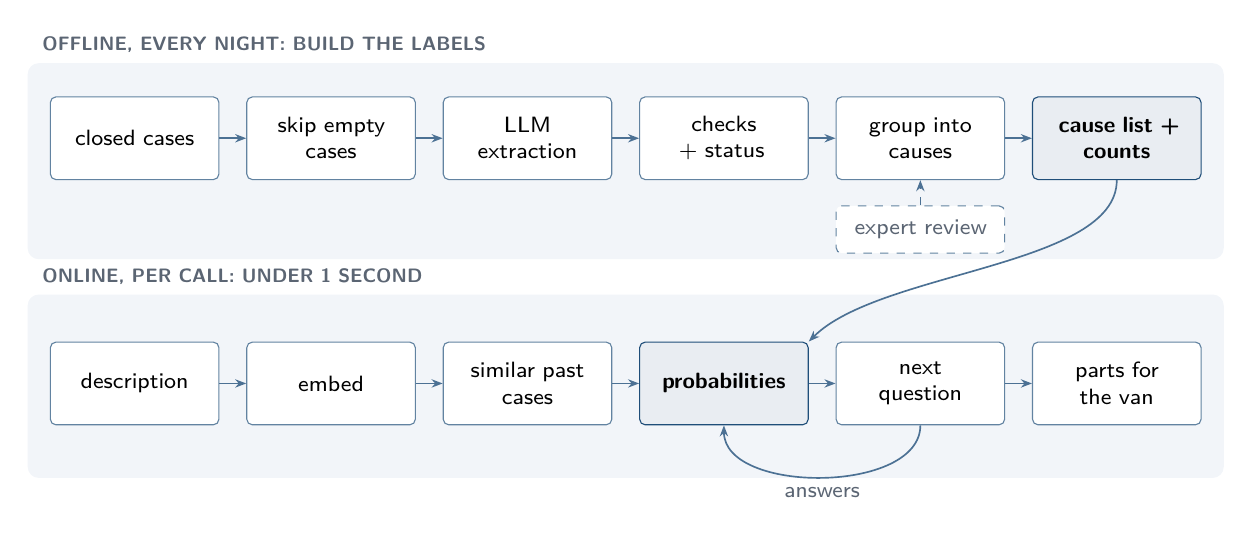
\begin{tikzpicture}[
    font=\sffamily\footnotesize,
    box/.style={draw=accent!70, fill=white, rounded corners=2pt, align=center, text width=2.0cm, minimum height=1.05cm, inner sep=2pt},
    hot/.style={box, fill=accent!10, draw=accent, font=\sffamily\footnotesize\bfseries},
    arr/.style={-{Stealth[length=4pt]}, accent!80, line width=0.6pt},
    node distance=0.34cm]
  \node[box] (cases) {closed cases};
  \node[box, right=of cases] (triage) {skip empty\\cases};
  \node[box, right=of triage] (extract) {LLM\\extraction};
  \node[box, right=of extract] (validate) {checks\\+ status};
  \node[box, right=of validate] (cluster) {group into\\causes};
  \node[hot, right=of cluster] (table) {cause list +\\counts};
  \node[box, below=0.32cm of cluster, dashed, minimum height=0.6cm, text=muted] (expert) {expert review};
  \foreach \a/\b in {cases/triage, triage/extract, extract/validate, validate/cluster, cluster/table} \draw[arr] (\a) -- (\b);
  \draw[arr, dashed] (expert) -- (cluster);
  \node[box, below=2.05cm of cases] (desc) {description};
  \node[box, right=of desc] (embed) {embed};
  \node[box, right=of embed] (knn) {similar past\\cases};
  \node[hot, right=of knn] (post) {probabilities};
  \node[box, right=of post] (question) {next\\question};
  \node[box, right=of question] (loadout) {parts for\\the van};
  \foreach \a/\b in {desc/embed, embed/knn, knn/post, post/question, question/loadout} \draw[arr] (\a) -- (\b);
  \draw[arr] (question.south) to[out=-90, in=-90, looseness=0.9] node[below, text=muted] {answers} (post.south);
  \draw[arr] (table.south) .. controls +(0,-1.1) and +(0.9,0.9) .. (post.north east);
  \begin{scope}[on background layer]
    \node[fit=(cases)(table)(expert), inner xsep=8pt, inner ysep=7pt, yshift=5pt, fill=wash, rounded corners=4pt] (off) {};
    \node[fit=(desc)(loadout), inner xsep=8pt, inner ysep=18pt, yshift=-1pt, fill=wash, rounded corners=4pt] (on) {};
  \end{scope}
  \node[anchor=south west, font=\sffamily\scriptsize\bfseries, text=muted] at ([xshift=2pt]off.north west) {OFFLINE, EVERY NIGHT: BUILD THE LABELS};
  \node[anchor=south west, font=\sffamily\scriptsize\bfseries, text=muted] at ([xshift=2pt]on.north west) {ONLINE, PER CALL: UNDER 1 SECOND};
\end{tikzpicture}
\end{center}

\textbf{The LLM reads, statistics decide.} The LLM turns messy, multilingual text into structured records. The probabilities are counted from similar past cases.

I considered two other options:
\begin{itemize}
  \item \textbf{Similar cases + an LLM that writes “causes with percentages”.} Quickest to build, but the numbers are not calibrated, change when you ask again, cannot be tested one by one, and the LLM call is too slow for a 3-second budget.
  \item \textbf{A trained classifier.} It needs the same labels, is weak on rare causes, and needs retraining as data grows. It can come later, on top of these labels.
\end{itemize}
The cost of my choice: two systems instead of one, and a cause list that someone has to own.

\subsection{Offline: turning closed cases into labels}\label{sec:offline}

This runs once over the 100k history, then every night for new cases.

\begin{enumerate}
  \item \textbf{Skip} cases with no technician notes and no resolution: there is no evidence of a cause.
  \item \textbf{Extract.} One LLM call per case returns JSON: the outcome (fixed, no fault found, warranty swap, not fixed, not technical), the failed component in short English, a \textbf{word-for-word quote} from the technician as evidence, the role of each replaced part, the customer's symptoms and any error codes.
  \item \textbf{Check.} Plain code checks every record. The quote must appear in the technician's text (allowing for ü/ue and accents), not in the customer's, and must say the part was at fault: “No oil leak found” and “Contactor tested OK” are not evidence. In English it must also name the component; other languages are flagged for a multilingual check. Every replaced part gets one role and no part is invented. The outcome must match the rest. Failures go to a review queue; they never quietly become labels.
  \item \textbf{Status.} Only fixed, checked cases are counted. Warranty swaps and billing calls are excluded. “No fault found” becomes its own cause per family, because dispatchers should see it. Temporary fixes are attached to a cause but not counted.
  \item \textbf{Group into causes}, per equipment family. My rule: \textbf{two cases have the same cause if the technician would bring the same parts and do the same repair.} “Main contactor” and “Hauptschütz” are one cause. A boom-cylinder seal kit (C-48604) and a whole new cylinder (C-48755) are two, even though both customers report a leak at the boom cylinder.

  The distance between two cases is 1 minus the text similarity of their English component. If both replaced parts and the parts are different, they can never merge. Shared parts bring them closer. Cases with no parts (cleaning, tightening) rely on the text alone:
  \[
  d(a,b) = \begin{cases}
    1 & \text{both replaced parts, none shared}\\
    \bigl(1 - \cos(a,b)\bigr)\bigl(1 - 0.5\,J(a,b)\bigr) & \text{parts shared ($J$: overlap of the part sets)}\\
    1 - \cos(a,b) & \text{otherwise}
  \end{cases}
  \]
  I use \textbf{complete-linkage clustering} with a cut at 0.4:
  \begin{itemize}
    \item k-means needs the number of causes, which we do not know.
    \item HDBSCAN treats small groups as noise, but for rare machine types the small groups are the real causes.
    \item Splitting one cause in two is cheaper: the same parts go on the van, and a reviewer merges them with one click. It is not free, because it halves the counts and takes two places in the list, so the nightly report flags causes fixed with the same parts as merge candidates. Merging two causes is expensive and silent. Complete linkage prefers to split.
  \end{itemize}
  It runs on the distinct (component, parts) wordings of a family, not on cases. The LLM writes short generic names, so I expect hundreds to a few thousand per family. Complete linkage keeps every pair in memory, about 0.4\,GB at 10k wordings, which is fine for a monthly job; the backfill logs the count per family. If a family outgrows this, it splits without changing the result: complete linkage never puts two wordings further apart than the cut into one cause, so no cause spans two groups of the “closer than 0.4” graph. A radius search finds those groups (at 0.8 on text alone, because shared parts can at most halve a distance), and each is clustered on its own.
  \item \textbf{New cases every night} join the nearest cause only if they are close and the choice is clear. Otherwise they go to a pool, which becomes \emph{proposed} causes for an expert. A new kind of failure is never forced into an old cause.
\end{enumerate}

A senior technician spends about a day per main family reviewing and naming the causes and entering minutes-to-check. After that, about 15 minutes a week on new proposals. I kept this step human on purpose.

\subsection{Online: from description to parts}\label{sec:online}

\begin{enumerate}
  \item Embed the description and find the 50 most similar past cases of the same machine type, with closer cases weighted more. If there are few, add cases from the wider family at half weight.
  \item Count the causes of those cases, and add the family average as a prior worth about five cases ($\alpha = 5$). This is how a rare type like the CX-300 borrows from the CX-450.
  \item Each answer updates the list with Bayes' rule, using $P(\text{answer} \mid \text{cause})$ (below). “Don't know” changes nothing. An answer the LLM pre-fills from the description is shown but does not update the list: the similar-case search already used that text, so counting it again would double the evidence.
  \item The next question, among those a customer can answer, is the one most likely to change the parts on the van: for each answer, re-run the loadout rule (step 5) on the updated list, and add up the probability of the answers that change it. This is the stopping test of 1.3 turned into a score. Information gain over causes would also ask questions that only separate causes needing the same parts (“only when cold?” in the walkthrough), so it only breaks ties, where it still helps the technician's check order.
  \item Stop and suggest the parts as described in 1.3. A temperature on the probabilities, fitted on the last month of cases, keeps them calibrated.
\end{enumerate}

\textbf{Where $P(\text{answer} \mid \text{cause})$ comes from at launch.} The old cases never recorded answers to my questions, and a customer who did not mention a repeat flat battery has not said “no”. So the history alone cannot give these numbers. It can choose the questions: they come from the customer symptoms the LLM extracted, grouped the same way, and a symptom mentioned far more often with one cause than across the family (“third time this month” with the alternator) becomes a candidate. Its mention rate is only a floor for $P(\text{yes} \mid c)$, because customers leave things out. The senior technician then fills in one row per question: for each cause, “usually yes”, “usually no” or “unrelated”, which I map to 0.8, 0.2 and the family's base rate. That estimate counts as 10 answers. Every answer logged in \code{diagnostic_session} with its confirmed cause is added on top, so after 30 answers for a cause the data carries three quarters of the weight. Until then, one answer may change a cause's odds by at most a factor of 4 either way, so a guessed number can move a cause but never remove it. In the walkthrough, the alternator's drop from 9\% to 2\% is one “no” at that limit. With at most three questions and this limit, treating answers as independent cannot run away. The cost: at launch the questions are only as good as the expert, and their value can only be measured from live sessions (section~\ref{sec:works}).

\begin{callout}
{\sffamily\bfseries In formulas}\par\smallskip
{\renewcommand{\arraystretch}{1.9}%
\begin{tabular}{@{}>{$\displaystyle}l<{$} >{\RaggedRight\arraybackslash}p{7.0cm}@{}}
w_i = \max\Bigl(0,\ \frac{s_i - s_0}{1 - s_0}\Bigr) & weight of neighbour $i$ ($s_i$: similarity; $s_0$: a floor set in the backtest) \\
p(c \mid d) \propto \sum_i w_i\,[\mathrm{cause}_i = c] + \alpha\,\pi_c & counts plus the family prior $\pi$, with $\alpha = 5$ \\
p(c \mid d, a) \propto p(c \mid d)\,P(a \mid c) & update after answer $a$ (Bayes) \\
P(\text{yes} \mid c) = \frac{k_c + 10\,\pi_{qc}}{n_c + 10} & expert estimate $\pi_{qc}$, worth 10 answers, plus $k_c$ “yes” of $n_c$ logged \\
\sum_c p(c)\,\bigl[\text{all usual parts of } c \in L\bigr] \ge 0.8 & van loadout $L(p)$: the smallest part set that reaches this coverage \\
q^{*} = \arg\max_q \sum_a P(a)\,\bigl[L(p_a) \ne L(p)\bigr] & next question: the one most likely to change the loadout ($p_a$: the list after answer $a$); information gain breaks ties \\
\end{tabular}}
\end{callout}

\textbf{Speed:} embedding 150\,ms + vector search 30\,ms + scoring under 10\,ms + network about 300\,ms, so \textbf{under 1 second}. The LLM is not on this path; its extras arrive after 2--5 seconds.

\subsection{Data}\label{sec:data}

Everything lives in Aurora PostgreSQL with pgvector (\code{sql/schema.sql}):
\begin{itemize}
  \item \textbf{\code{case_record}}: one row per closed case. The example below is C-48590, as the pipeline produced it (shortened).
  \item \textbf{\code{cause}}: the cause list (approved, proposed or retired), with minutes-to-check.
  \item \textbf{\code{cause_exemplar}}: the different wordings of each cause, used to match new cases.
  \item \textbf{Count tables}: refreshed every night and kept in memory by the API.
  \item \textbf{\code{diagnostic_session}}: what was shown, the answers, the parts and the confirmed cause. This is a free test set.
\end{itemize}

\begin{Verbatim}
{"case_id": "C-48590", "equipment_type": "CX-450", "language": "en",
 "symptom_text": "no crank, dead panel", "outcome_type": "fixed",
 "label_status": "trusted", "cause_id": "air-compressor-cx/frame-ground-strap",
 "component": "frame ground strap", "certainty": "observed",
 "evidence_quote": "Ground strap at frame was loose, heavy corrosion.",
 "parts": [], "extractor_version": "extract-v1/<model-id>"}
\end{Verbatim}

A new case is matched by vector search over the old \emph{customer descriptions}, filtered by customer, machine type and status. Customer text is what we have at intake. 100k vectors are about 0.4\,GB, so one database is enough.

\subsection{Processing and cost}\label{sec:processing}

\begin{itemize}
  \item \textbf{Backfill (once):} export to S3, then 10 batches of 10k cases through the LLM's batch API (half price, usually under an hour), then checks, embeddings and clustering. About \$0.7--1k. The slow part is the expert review: a few days.
  \item \textbf{Daily:} at 02:00 the same pipeline runs on about 500 new cases (about \$4--5), assigns them, and publishes quality metrics. New cases are searchable the next morning.
  \item \textbf{Weekly / monthly:} the pool becomes proposals every week. A full re-cluster runs monthly as a check and is never applied automatically.
  \item \textbf{Running cost:} about \$600 a month for one customer (database \$150, compute \$60, daily extraction \$130, online LLM text \$250), plus about \$1k once. The online LLM text is optional and is the first thing to cut if cost matters.
\end{itemize}

\subsection{What can go wrong, and how I would notice}\label{sec:failures}

{\small
\begin{longtable}{@{}R{0pt}{2} R{0pt}{2}@{}}
\toprule
Problem & How I would notice \\
\midrule
\endhead
\bottomrule
\endfoot
The LLM invents a cause, or takes the customer's guess & Quote check; review rate per family and language; the share of labels whose quote is not yet checked against the component, per language (all non-English ones for now); a monthly hand check of 50 cases, half of them non-English \\
A warranty swap becomes a fake cause & A whole-unit part with outcome “fixed” goes to review; outcome mix over time \\
Two causes merged into one & Parts purity: under 80\% of the members share the same fix part \\
One cause split in two, often by language & Two causes in a family fixed with the same parts; or all members in one language while the family is mixed (chance below 5\%) \\
A new kind of failure & The pool of unassigned cases keeps growing \\
Counts favour causes fixed on the first visit: not-fixed cases are left out, so the causes that cost a second visit look rarer & Per family, compare each cause's share among provisional (not-fixed) cases with its share among counted ones; an asset ID would let me count the return visit \\
Probabilities too confident & Compare the list shown at dispatch with the confirmed cause; alert when calibration error goes above 0.05 \\
Feedback loop: the suggested part is swapped just because it was on the van & More “swapped” and fewer “measured” causes over time; 4 weeks of shadow mode as a baseline \\
\end{longtable}
}

\subsection{Stack (AWS)}\label{sec:stack}

\begin{itemize}[itemsep=0.35em]
  \item \textbf{Frontend:} a React + TypeScript component inside the existing dispatcher screen, and the same component as a phone web app (PWA) that works offline. Nobody switches tabs during a call, and basements have no signal. Downside: releases are tied to the host app.
  \item \textbf{API:} FastAPI (Python) on ECS Fargate, with the counts in memory. It shares code with the pipeline. Many customers would need a cache such as ElastiCache.
  \item \textbf{Data:} Aurora PostgreSQL + pgvector, and S3 for exports. One store is enough up to about 10M vectors; after that, OpenSearch.
  \item \textbf{LLM:} Claude Opus 5.5 through Claude Platform on AWS, for AWS billing, IAM and the batch API. It is the model of the real run in section~\ref{sec:built}. EU data residency needs checking; Bedrock in eu-central-1 is the fallback.
  \item \textbf{Embeddings:} Cohere Embed Multilingual v3 on Bedrock, which puts German, English, French and Italian in one space. Abbreviations embed badly, so I also embed the LLM's English summary.
  \item \textbf{Jobs:} EventBridge \ra{} Step Functions \ra{} Lambda and Fargate. Waiting hours for a batch is a normal Step Functions wait.
\end{itemize}

% ================================================================ 3
\section{What I built: the label factory}\label{sec:built}

\textbf{Why this part.} Everything else uses well-known methods: embeddings, vector search, counting, information gain. But all of it depends on cause labels that do not exist in this data, and mistakes in them are invisible. Merged causes put the wrong parts on the van with high confidence. Causes split by language halve the evidence. Warranty swaps become fake diagnoses. The online system and its evaluation would both be wrong in the same way. So this is the part that can break the whole system without anyone noticing.

\textbf{What is in the code} (\code{src/diagnostic_assist/labeling/}; the README lists every file):
\begin{itemize}
  \item \textbf{Built:} the prompt and JSON schema, a single-call LLM extractor and recorded replay, the checks, the status logic, the clustering, the nightly assignment and the quality checks. I had no API key, so the recorded run (\code{scripts/record_extractions.py}) sends the same prompt and schema through the Claude Code CLI; the SDK extractor itself has not run.
  \item \textbf{Stubbed}, each with a note on the real version: the ERP parts catalogue, the Bedrock embedder (a simple word-based embedder stands in), the batch extraction for the backfill, and keeping cause IDs stable after a re-cluster.
  \item \textbf{Not built:} storage, orchestration and the online scorer.
\end{itemize}

\textbf{Results on the 22 sample cases, from the real model} (\texttt{python scripts/run\_labeling.py}). I ran the extraction prompt through Claude Opus 5.5 at low effort: one call per case, so the model never saw two cases together, with tools off and no project context. The run cost \$0.30, about \$0.014 a case at list price, which puts the backfill at about \$0.7k through the batch API, as in section~\ref{sec:processing}.
\begin{itemize}
  \item 18 trusted, 1 no fault found, 3 excluded, none held for review. The 18 form 14 causes, grouped exactly like my hand labels (B-cubed precision and recall 1.00).
  \item The English/German contactor, English/Italian valve plate and English/German conrod bearing cases each became one cause. The seal kit and the whole cylinder stayed apart. The “oil puddle” case was labelled as the condensate drain line, and “battery dead again” as the alternator.
  \item Against my hand-written extractions: outcome, part roles and error codes matched in all 22 cases. The component was worded differently in 4 (“compressor valve plate”, “schrader valve” with the suction line as its location), and the clustering absorbed all of them. A second run gave the same outcome, component and parts in all 22 cases; only mechanism, certainty or location changed, in 4 cases, and none of those feeds the status or the clustering.
  \item In a night-by-night test, a new German bearing case joined the cause first formed from an English case, and new failure types arrived as proposals.
\end{itemize}

\textbf{The one disagreement was useful.} For the temporary fix C-48801 (“temp fix w/ sealant, ordered seal kit”) I had written a provisional cause; the model returned none, so the case is excluded instead of provisional. My prompt allows both readings: rule 2 says no quote means no cause, while rule 6 asks for a provisional cause “if one is stated”. Ordering a seal kit names the part for the next visit, not what failed, so I side with the model. I left the prompt unchanged so that it still matches the recorded run; changing rule 6 is the first step in section~\ref{sec:next}. It costs nothing in the counts, because provisional cases are never counted, and the outcome “not fixed”, my first-time-fix proxy, was right. Writing the extractions by hand could not have found this.

\textbf{What this does not show.} The extraction is now real, but these 22 cases are clean: nothing reached review, so the checks have not yet met a real model error (the review example below is written by hand). The gold labels are still mine. The threshold sweep (\texttt{scripts/evaluate\_against\_gold.py}) cannot choose a cut either: with the parts rule anything from 0.1 to 0.9 works, on text alone only 0.2--0.5. I keep 0.4 so it is safe even when a case has no parts.

\textbf{New cases} (\texttt{python scripts/label\_case.py examples/*.json}): a French CX-300 contactor case joins the contactor cause; a tank safety valve becomes a proposed new cause; and a bad extraction that took the cause from the customer's “Ölfleck” (oil stain) is held for review.

\begin{callout}
The safety valve also showed a real weakness. By text it is only 0.32 from “reed valve”, inside the cut. Only the different parts kept them apart. A safety valve that was adjusted without a new part would land in the wrong cause. Item~8 in section~\ref{sec:next} deals with this.
\end{callout}

% ================================================================ 4
\section{How I would know it works}\label{sec:works}

\textbf{(a) Are the labels right?} Two senior technicians label 400 cases on their own, spread over the main families, languages and outcomes, plus 50 rare ones. I measure how much they agree (Cohen's $\kappa$), how accurate the extraction is, and how well my clusters match theirs (B-cubed). \emph{Stop if} $\kappa$ is below 0.6: the experts do not agree what a cause is, so the cause list itself is wrong. Also stop if B-cubed precision is below 0.9: causes are being merged.

\textbf{(b) Are the probabilities useful?} Build everything from cases before a given month, and predict that month from the customer text alone. Measure whether the true cause is in the top 3, how well calibrated the numbers are, and how often the suggested parts covered what was actually replaced. Compare with “load what usually breaks on this model”. \emph{Stop if} that simple baseline is not beaten by at least 10 points: then the text does not carry enough signal. Old cases have no answers to my questions, so the backtest cannot score them. Shadow mode cannot either, because nobody sees the questions. I measure them in the rollout of (c), by comparing the parts suggested before and after the answers in each session, and \emph{drop the questions} if two of them add less than 5 points to how often the van had the parts that were used.

\textbf{(c) Does it improve first-time fixes?} Four weeks in shadow mode (logged, not shown), then a rollout split by dispatcher team. Seeing +3 points over a 75\% first-time-fix rate needs about 3,300 cases per group, which is about two weeks of volume. Because the split is by team, cases within a team are alike and count for less: the 3,300 grows by $1 + (m-1)\rho$, for $m$ cases per team and a within-team correlation $\rho$. I would measure $\rho$ in the shadow weeks and size the test from it, which is why I plan 4--6 weeks, not two. \emph{Stop if} nothing improves, or if dispatchers change the suggested parts in more than half of the calls.

To measure first-time fix properly we need an asset or serial number to link repeat visits. The data has none. Until then, the “not fixed” outcome rate is the proxy. That ID is my first request to the business.

% ================================================================ 5
\section{What I cut}\label{sec:cut}

\begin{itemize}[itemsep=0.3em]
  \item \textbf{Asset history.} There is no asset ID, so repeat visits (“third time this month”) cannot be linked. This is probably a strong signal; it needs data, not code.
  \item \textbf{The online scorer.} Designed (2.3), not built. It is standard, and useless without good labels.
  \item \textbf{The question bank.} Same clustering, the next step once the labels are trusted.
  \item \textbf{Smarter check ordering} than probability divided by minutes.
  \item \textbf{Images and voice notes.} Voice notes would probably improve the notes the most, but they are out of scope.
  \item \textbf{Fine-tuned models.} Not before there are about 50 trusted cases per cause.
  \item \textbf{Links between families, and a cause hierarchy.} Later, once the expert review shows where they help.
  \item \textbf{Personal data and data residency.} \code{tenant_id} is in every table, but removing names and phone numbers before the LLM, and a legal check on where data is stored, are needed before production.
  \item \textbf{Automatic changes to the cause list.} Cut on purpose: re-clustering only proposes; a person decides.
\end{itemize}

% ================================================================ 6
\section{What I would do with more time}\label{sec:next}

In order of risk: first check the labels on real data, then build what uses them.

\begin{enumerate}[itemsep=0.3em]
  \item \textbf{Scale the real extraction run} from 22 to 2,000 cases across families and languages, after fixing rule 6 of the prompt, and check 100 by hand. It is the first test of the checks against real model errors.
  \item \textbf{Build the 400-case gold set} with two technicians. A spreadsheet is enough.
  \item \textbf{Add the real embedder} (Cohere on Bedrock) and choose the threshold on the gold set, starting with no-part fixes. Use it, or a second small LLM call that sees only the quote and the component, to check that non-English quotes name the component.
  \item \textbf{Build the question bank} from the extracted symptoms, reviewed by the expert.
  \item \textbf{Build the backtest} from section~\ref{sec:works}(b), with the “usual parts” baseline.
  \item \textbf{Build the online scorer} (FastAPI, pgvector, counts in memory), with tests that probabilities add up to 1 and that “don't know” changes nothing. Only if the backtest says it is worth it.
  \item \textbf{Storage, Step Functions and a small review tool} to merge, split and name causes.
  \item \textbf{If nightly matching falls below 95\% precision}, especially for no-part fixes, add an LLM step that picks from the top five causes or says “none”.
  \item \textbf{Before production:} remove personal data before the LLM, confirm data residency, and get an asset ID.
\end{enumerate}

% ================================================================ 7
\section{Where I used AI, and where I overrode it}\label{sec:ai}

\textbf{Where I used it.} I used Claude Opus 5.5 (through Claude Code) for most of the typing: first drafts of the code and the tests, checking my reading of the German and French technician notes, and turning my notes into clear English and \LaTeX. I read, ran and changed everything it wrote. The decisions in this document are mine: what counts as one cause, which checks block a label, the merge threshold, and what to cut. The real extraction run in section~\ref{sec:built} also used Claude Opus 5.5, through the Claude Code CLI because I had no API key. There the model was the system under test, not a helper: each call saw one case and the prompt, and nothing else.

\textbf{Where I overrode it.}
\begin{enumerate}
  \item \textbf{Clustering.} The model suggested HDBSCAN, because the number of causes is unknown. I chose complete-linkage with a distance cut instead. HDBSCAN treats small groups as noise, but on a rare machine type, two cases can be a real cause. Also, splitting one cause in two is easy to fix later, while merging two different causes is silent.
  \item \textbf{What the LLM is allowed to decide.} The model's first design let the LLM read a case and return the root cause and its probability directly. I limited the LLM to reading: it turns text into a structured record, and plain code checks that record against the case. The probabilities come from counting similar past cases, because an LLM that makes up a number gives no sign when it is wrong.
\end{enumerate}

\end{document}
